{AOE(Activity On Edge
network)网的{边表示活动,边有权值代表活动持续时间,顶点表示事件,事件是图中新活动开始或者旧活动结束的标志。}}

{在AOE网络中,{\textbf{从源点到汇点的所有路径中,具有最大路径长度的路径称为关键路径}}。关键路径代表了整个工程所完成的\textbf{{最短时间}}。这么理解吧,工程的各个段是可以并行进行的,即使这个工程并行程度足够高,最长路径代表了工程至少需要的完成时间。}

{求关键路径的一般方法:}

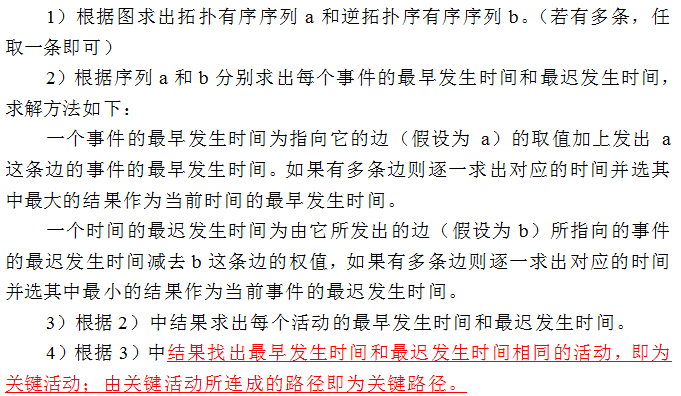
\includegraphics[width=3.70833in,height=2.15625in]{png-jpeg-pics/E7061CD56D902F653AFC2CAED02064D4.png}
